\documentclass[11pt]{beamer}
\beamertemplatenavigationsymbolsempty
\usetheme{Berlin}
\usecolortheme{default}
\setbeamerfont{frametitle}{size=\Large}
\setbeamertemplate{frametitle}[default][center]
\usefonttheme[onlymath]{serif}
% \useoutertheme{infolines}

\usepackage{amsmath}
\usepackage{amssymb}
\usepackage{graphicx}
\usepackage{tikz}
\usepackage{pgfplots}
\usepackage{pgfplotstable}
\usepackage{siunitx}
\usepackage{hyperref}
\usepackage{listings}
\usepackage{color}
\usepackage{verbatim}
\usepackage{subcaption}
\usepackage{multicol}
\usepackage{multirow}
\usepackage{booktabs}
\usepackage{array}
\usepackage{tabularx}
\usepackage{bm}
\usepackage{physics}


\newcommand{\itemb}{\item[$\bullet$]}
\newcommand{\itemw}{\item[$\circ$]}



\title{Using quantum annealing for equilibrium quantum simulation}
\author{Vid Eržen\\Advisor: Prof. Dr. Dragan Mihailović\\Co-advisor: Dr. Jaka Vodeb}
\date{April 24, 2024}

\begin{document}

\begingroup
    \setbeamertemplate{footline}{}
    \begin{frame}
        \titlepage
    \end{frame}
\endgroup

\setbeamertemplate{footline}[frame number]

\section{Introduction}
\begin{frame}
    \frametitle{Introduction}
    \begin{enumerate}
        \setlength{\itemindent}{-1em}
        \item introduction
        \item universality of Ising model
        \item quantum annealing
        \item equilibrium quantum simulation
        \item conclusion
    \end{enumerate}
\end{frame}

\begin{frame}
    \frametitle{Motivation}
    \begin{itemize}
        \setlength{\itemindent}{-1em}
        \itemb magnetic phase diagrams in quantum systems
        \begin{itemize}
            \setlength{\itemindent}{-1em}
            \item [-] Heisenberg model
            \item [-] transverse field Ising model (TFIM)
        \end{itemize}
        \itemb universal quantum computers currently too small $\to$ specialized
        \item [] quantum simulators
        \begin{itemize}
            \setlength{\itemindent}{-1em}
            \item [-] quantum annealing
        \end{itemize}
    \end{itemize}
\end{frame}

\begin{frame}
    \frametitle{Quantum annealing and gate model}
    \begin{itemize}
        \setlength{\itemindent}{-1em}
        \itemb computation: programmable transformation input $\to$ output.
    \end{itemize}
    \vspace*{0.3cm}
    \begin{columns}[T]
        \begin{column}{0.45\textwidth}
            \centering
            \textbf{Gate model} \\
            \hrulefill \\
            \begin{itemize}
                \item [-] digital (series of quantum gates)
                \item [-] universal
            \end{itemize}
            \begin{figure}[!htb]
                \centering
                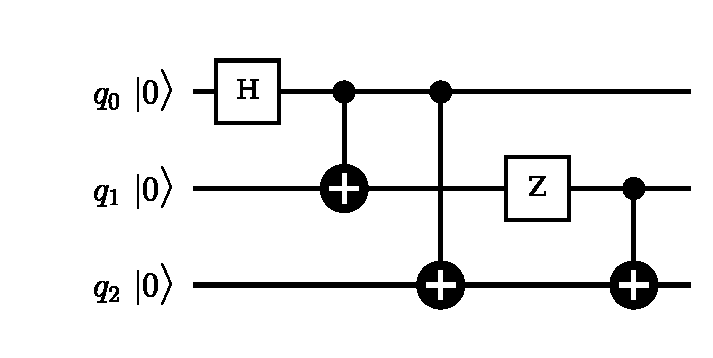
\includegraphics[width=\textwidth]{../plots/quantum_circuit.pdf}
                \label{fig:circuit}
            \end{figure}
        \end{column}
        \begin{column}{0.55\textwidth}
            \centering
            \textbf{Quantum annealing} \\
            \hrulefill \\
            \begin{itemize}
                \item [-] analog (programmable time-dependent Hamiltonian)
                \item [-] universality Hamiltonian-dependent
            \end{itemize}
            \begin{figure}[!htb]
                \centering
                \vspace*{-0.3cm}
                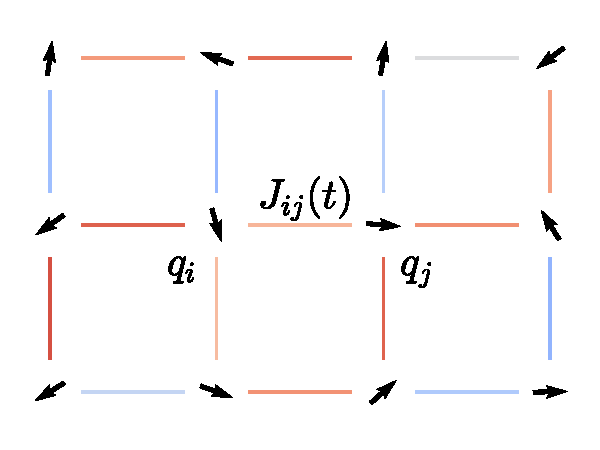
\includegraphics[width=0.65\textwidth]{../plots/lattice.pdf}
                \label{fig:annealing}
            \end{figure}
        \end{column}
    \end{columns}
\end{frame}

\begin{frame}
    \frametitle{Quantum annealing in practice}
    \begin{itemize}
        \setlength{\itemindent}{-1em}
        \itemb D-Wave Systems quantum annealers only implement the
        \item [] transverse Field Ising Model (TFIM)
        \begin{equation*}
            H =  - \Gamma \sum_i \sigma_i^x + \sum_{\expval{i,j}} J_{ij} \sigma_i^z \sigma_j^z + \sum_i h_i \sigma_i^z
            \label{eq:tfim}
        \end{equation*}
        \begin{itemize}
            \setlength{\itemindent}{-2em}
            \item[-] good for optimization problems
            \item[-] not general enough for universal quantum computation
            \item[-] limited number of simulable physical models
            \item[-] quantum Monte Carlo (QMC) methods efficient for equilibrium
            \item [] simulations of TFIM
        \end{itemize}
    \end{itemize}
\end{frame}


\section{Universality of Ising model}

\begin{frame}
    \frametitle{Optimization problems}
    \begin{itemize}
        \setlength{\itemindent}{-1em}
        \itemb example: graph partitioning problem
        \begin{figure}[!htb]
            \centering
            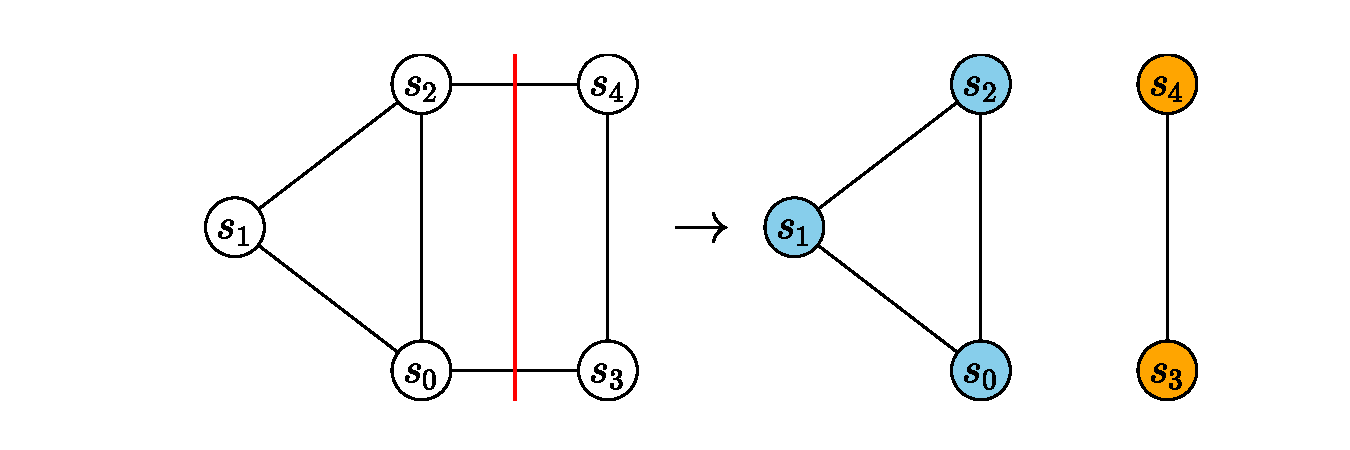
\includegraphics[width=0.7\textwidth]{../plots/max_cut_instance.pdf}
            \label{fig:graph_partitioning}
        \end{figure}
        \begin{enumerate}
            \setlength{\itemindent}{-2em}
            \item spin variable
            $
            s_i = \begin{cases}
                1 & \text{if } i \in A \\
                -1 & \text{if } i \in B
            \end{cases}
            $
            \vspace*{0.2cm}
            \item minimize number of edges between $A$ and $B$
            $$H = \sum_{(ij) \in V} \frac{1 - s_i s_j}{2}$$
        \end{enumerate}
    \end{itemize}
\end{frame}

\begin{frame}
    \frametitle{Universality of Ising model}
    \begin{columns}[T]
        \begin{column}{0.6\textwidth}
            \begin{itemize}
                \itemb finding the ground state of an Ising model = solving optimization problems
                \begin{itemize}
                    \item [-] search engine ranking
                    \item [-] travelling salesman problem
                    \item [-] scheduling problems
                \end{itemize}
                \vspace*{0.3cm}
                \begin{equation*}
                    H_P = \sum_{i,j} J_{ij} s_i s_j + \sum_i h_i s_i
                    \label{eq:ising}
                \end{equation*}
                \begin{itemize}
                    \item [-] $J_{ij}$ and $h_i$ specify the problem
                    \item [-] $\{s_i = \pm 1\}$ encodes the solution
                \end{itemize}
            \end{itemize}
        \end{column}
        \begin{column}{0.4\textwidth}
            \vspace*{1cm}
            \begin{figure}[!htb]
                \centering
                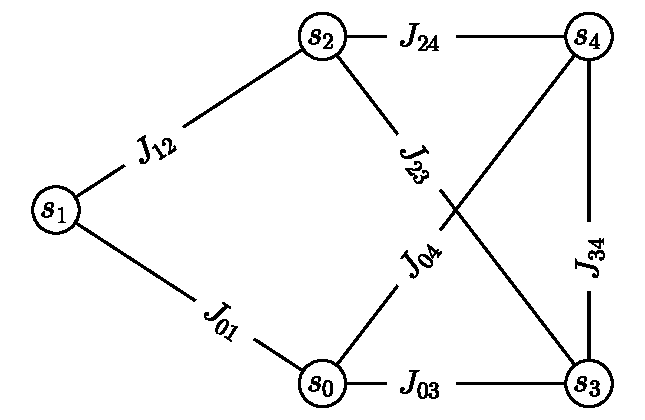
\includegraphics[width=\textwidth]{../plots/graph_instance.pdf}
                \label{fig:ising}
            \end{figure}
        \end{column}
    \end{columns}
\end{frame}


\section{Quantum annealing}

\begin{frame}
    \frametitle{Can quantum mechanics help us?}
    \begin{figure}[!htb]
        \centering
        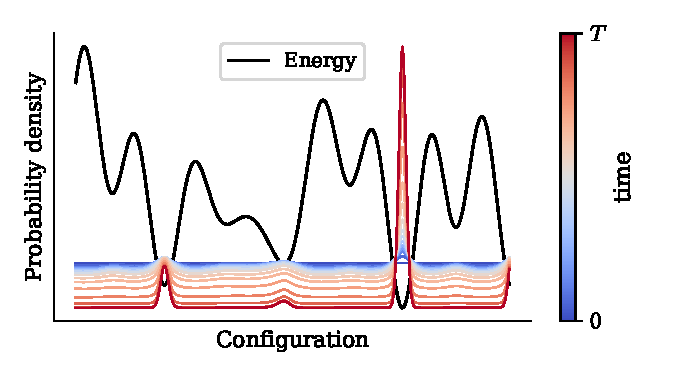
\includegraphics[width=0.7\textwidth]{../plots/QA.pdf}
        \label{fig:ising_gap}
    \end{figure}
\end{frame}

\begin{frame}
    \frametitle{Quantum adabatic theorem}
    \begin{block}{Adiabatic theorem}
        If a quantum system is prepared in the ground state of a Hamiltonian $H_0$
        and the Hamiltonian is changed slowly enough to $H_P$, the system will end up in the ground state of $H_P$.
    \end{block}
    \begin{columns}[T]
        \begin{column}{0.55\textwidth}
            \begin{itemize}
                \itemb interpolating Hamiltonian from $H_0$ to $H_P$
                in time $T$ (dimensionless time $s = t/T$)
                \begin{equation*}
                    H(s) = A(s) \, H_0 + B(s) \, H_P
                \end{equation*}
            \end{itemize}
        \end{column}
        \begin{column}{0.45\textwidth}
            \begin{figure}[!htb]
                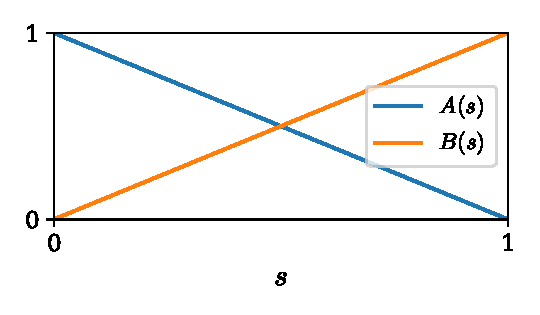
\includegraphics[width=\textwidth]{../plots/interpolating_functions.pdf}
            \end{figure}
        \end{column}
    \end{columns}
\end{frame}

\begin{frame}
    \frametitle{Quantum adiabatic theorem}
    \begin{columns}[T]
        \begin{column}{0.52\textwidth}
            \begin{itemize}
                \itemb interpolating Hamiltonian ($s = t/T$): $$H(s) = A(s) \, H_0 + B(s) \, H_P$$
                \itemb adiabatic theorem, specifically ($\hbar = 1$)
            \end{itemize}
        \end{column}
        \begin{column}{0.47\textwidth}
            \begin{figure}[!htb]
                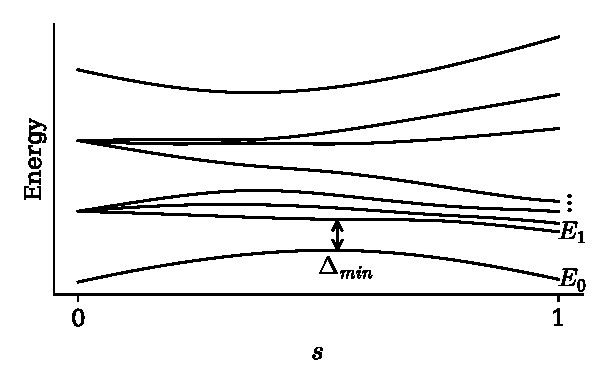
\includegraphics[width=\textwidth]{../plots/ising_gap.pdf}
            \end{figure}
        \end{column}
    \end{columns}
    \vspace*{-1em}
    \begin{equation*}
        T \gg \max_{0 \leq s \leq 1} \frac{\left| \mel{1(s)}{\frac{\partial H}{\partial s}}{0(s)} \right|}{\Delta(s)^2}
        \implies \left\vert{\braket{0(s = 1)}{\psi(s = 1)}}\right\vert^2  \approx 1
    \end{equation*}
\end{frame}

\begin{frame}
    \frametitle{Initial Hamiltonian}   
    \begin{itemize}
        \setlength{\itemindent}{-1em}
        \itemb requirements:
        \begin{itemize}
            \setlength{\itemindent}{-1em}
            \item [-] operates on two-state quantum systems --- qubits
            \item [-] easy to prepare its ground state experimentally
            \item [-] must not commute with $H_P = \sum_{\expval{i,j}} J_{ij} \sigma_i^z \sigma_j^z + \sum_i h_i \sigma_i^z$
        \end{itemize}
    \end{itemize} 

    \begin{columns}[T]
        \begin{column}{0.5\textwidth}
            \begin{itemize}
                \vspace*{1em}
                \itemb transverse field Hamiltonian 
                $$H_0 = - \sum_i \sigma_i^x$$
                \vspace*{-1.5em}
                \begin{itemize}
                    \item [-] ground state \\ \vspace*{0.5em} $\ket*{+++...} = \Pi_i^N \frac{\ket*{0}_i + \ket*{1}_i}{\sqrt{2}}$
                \end{itemize}
            \end{itemize}
        \end{column}
        \begin{column}{0.5\textwidth}
            \begin{figure}[!htb]
                \centering
                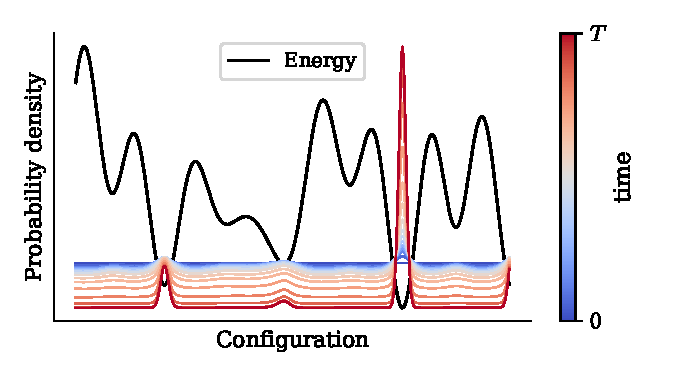
\includegraphics[width=\textwidth]{../plots/QA.pdf}
            \end{figure}
        \end{column}
    \end{columns}
\end{frame}

\begin{frame}
    \frametitle{Annealing Hamiltonian}
    \begin{itemize}
        \setlength{\itemindent}{-1em}
        \itemb full quantum annealing Hamiltonian = transverse field Ising 
        \item [] model (TFIM)
    \end{itemize}
    \begin{equation*}
        H(s) = - A(s) \sum_i \sigma^x_i + B(s) \left( \sum_i h_i \sigma^z_i + \sum_{i,j} J_{ij} \sigma^z_i \sigma^z_j \right)
    \end{equation*}
    \begin{columns}
        \begin{column}{0.6\textwidth}
            \vspace*{-1.5em}
            \begin{figure}[!htb]
                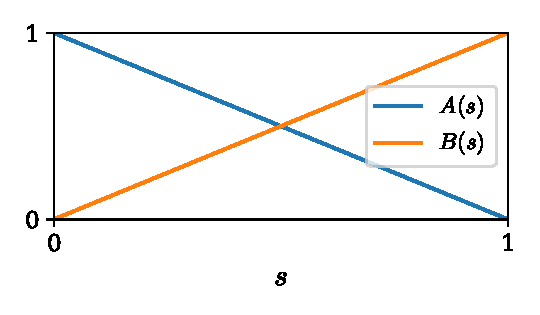
\includegraphics[width=0.7\textwidth]{../plots/interpolating_functions.pdf}
            \end{figure}
            \vspace*{-3em}
            \begin{figure}[!htb]
                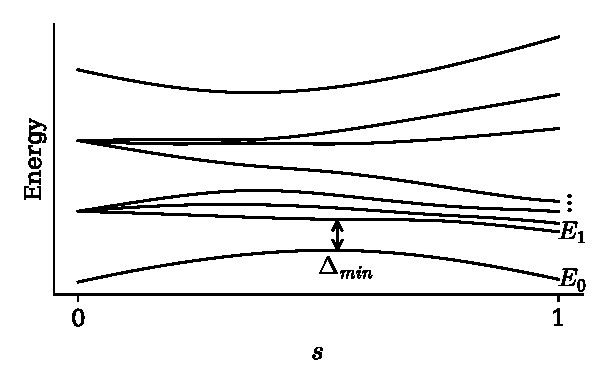
\includegraphics[width=0.7\textwidth]{../plots/ising_gap.pdf}
            \end{figure}
        \end{column}
        \begin{column}{0.4\textwidth}
            \vspace*{-2em}
            \begin{figure}[!htb]
                \hspace*{-2em}
                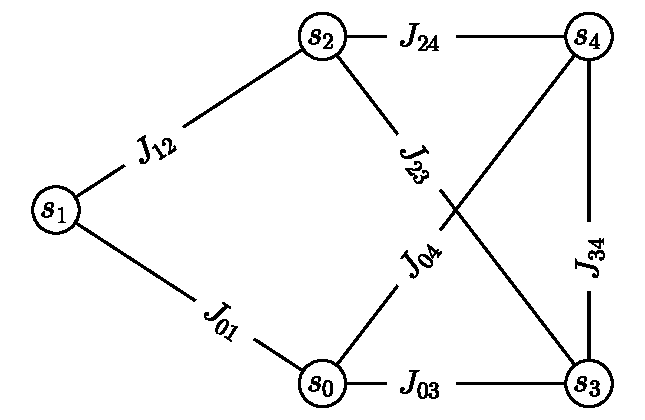
\includegraphics[width=\textwidth]{../plots/graph_instance.pdf}
            \end{figure}
        \end{column}
    \end{columns}
\end{frame}

\begin{frame}
    \frametitle{Annealing schedule}
    \begin{itemize}
        \setlength{\itemindent}{-1em}
        \itemb adiabatic theorem: proceed slowly when the gap is small and
        \item [] quickly when the gap is large
        \begin{itemize}
            \setlength{\itemindent}{-1em}
            \item [-] $s = t/T \to$ customizable function $s(t)$ (annealing schedule)
        \end{itemize}
    \end{itemize}
    \begin{figure}[!htb]
        \centering
        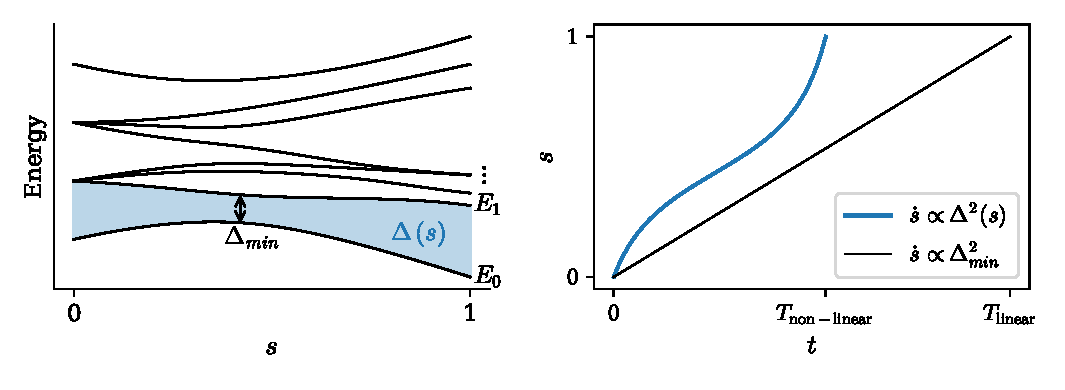
\includegraphics[width=0.9\textwidth]{../plots/ising_gap_with_annealing_schedule.pdf}
    \end{figure}
\end{frame}

\begin{frame}
    \frametitle{Overview}    
    \begin{itemize}
        \setlength{\itemindent}{-1em}
        \itemb solving optimization problems = finding the ground state of an
        \item [] Ising model
        \begin{itemize}
            \setlength{\itemindent}{-1em}
            \item[-] $\{J_{ij}, h_i\}$ specify the problem
        \end{itemize}
        \itemb annealing Hamiltonian = Ising + transverse field
        \begin{itemize}
            \setlength{\itemindent}{-1em}
            \item [-] parts must not commute $\to$ transitions between states
            \item [-] initial ground state as simple as possible
        \end{itemize}
        \begin{equation*}
            H(s) = - A(s) \sum_i \sigma^x_i + B(s) \left( \sum_i h_i \sigma^z_i + \sum_{i,j} J_{ij} \sigma^z_i \sigma^z_j \right)
        \end{equation*}
        \itemb customizable annealing schedule $s(t)$
    \end{itemize}
\end{frame}


\section{Equilibrium quantum simulation}

\begin{frame}
    \frametitle{Equilibrium quantum simulation}
    \begin{itemize}
        \setlength{\itemindent}{-1em}
        \itemb phase diagram: How does a system behave at different
        \item [] parameters?
        \begin{itemize}
            \setlength{\itemindent}{-1em}
            \item [-] temperature $T$ 
            \item [-] magnetic field $h_i$
            \item [-] transverse field $A(s)$
        \end{itemize}
        \itemb system with eigenstates $\{\ket{\psi_n}\}$ and eigenenergies $\{E_n\}$ at
        \item [] temperature $T$
        \begin{equation}
            p_i = e^{-E_i/T} / Z
            \label{eq:boltzmann}
        \end{equation}
        \itemb Monte Carlo methods: draw $N$ samples $\{ s_i \}$ from \eqref{eq:boltzmann} and
        \item [] estimate observable $O$
        $$\expval{O} := \sum_i p_i \mel{\psi_i}{O}{\psi_i} \underset{N \to \infty}{\approx} \frac{1}{N} \sum_{n=1}^N O(s_n)$$
    \end{itemize}
\end{frame}

\begin{frame}
    \frametitle{Physical implementation of quantum annealers}    
    \begin{columns}[T]
        \begin{column}{0.5\textwidth}
            \begin{itemize}
                \itemb isolated systems
                \begin{itemize}
                    \item [-] deterministic evolution
                    \item [-] no temperature!
                \end{itemize}
                \vspace*{0.3cm} 
                \itemb physical devices couple with their environment at temperature $T$
                \begin{itemize}
                    \item [-] system thermalizes to $T$
                \end{itemize}
            \end{itemize}
            \begin{figure}
                \vspace*{-1em}
                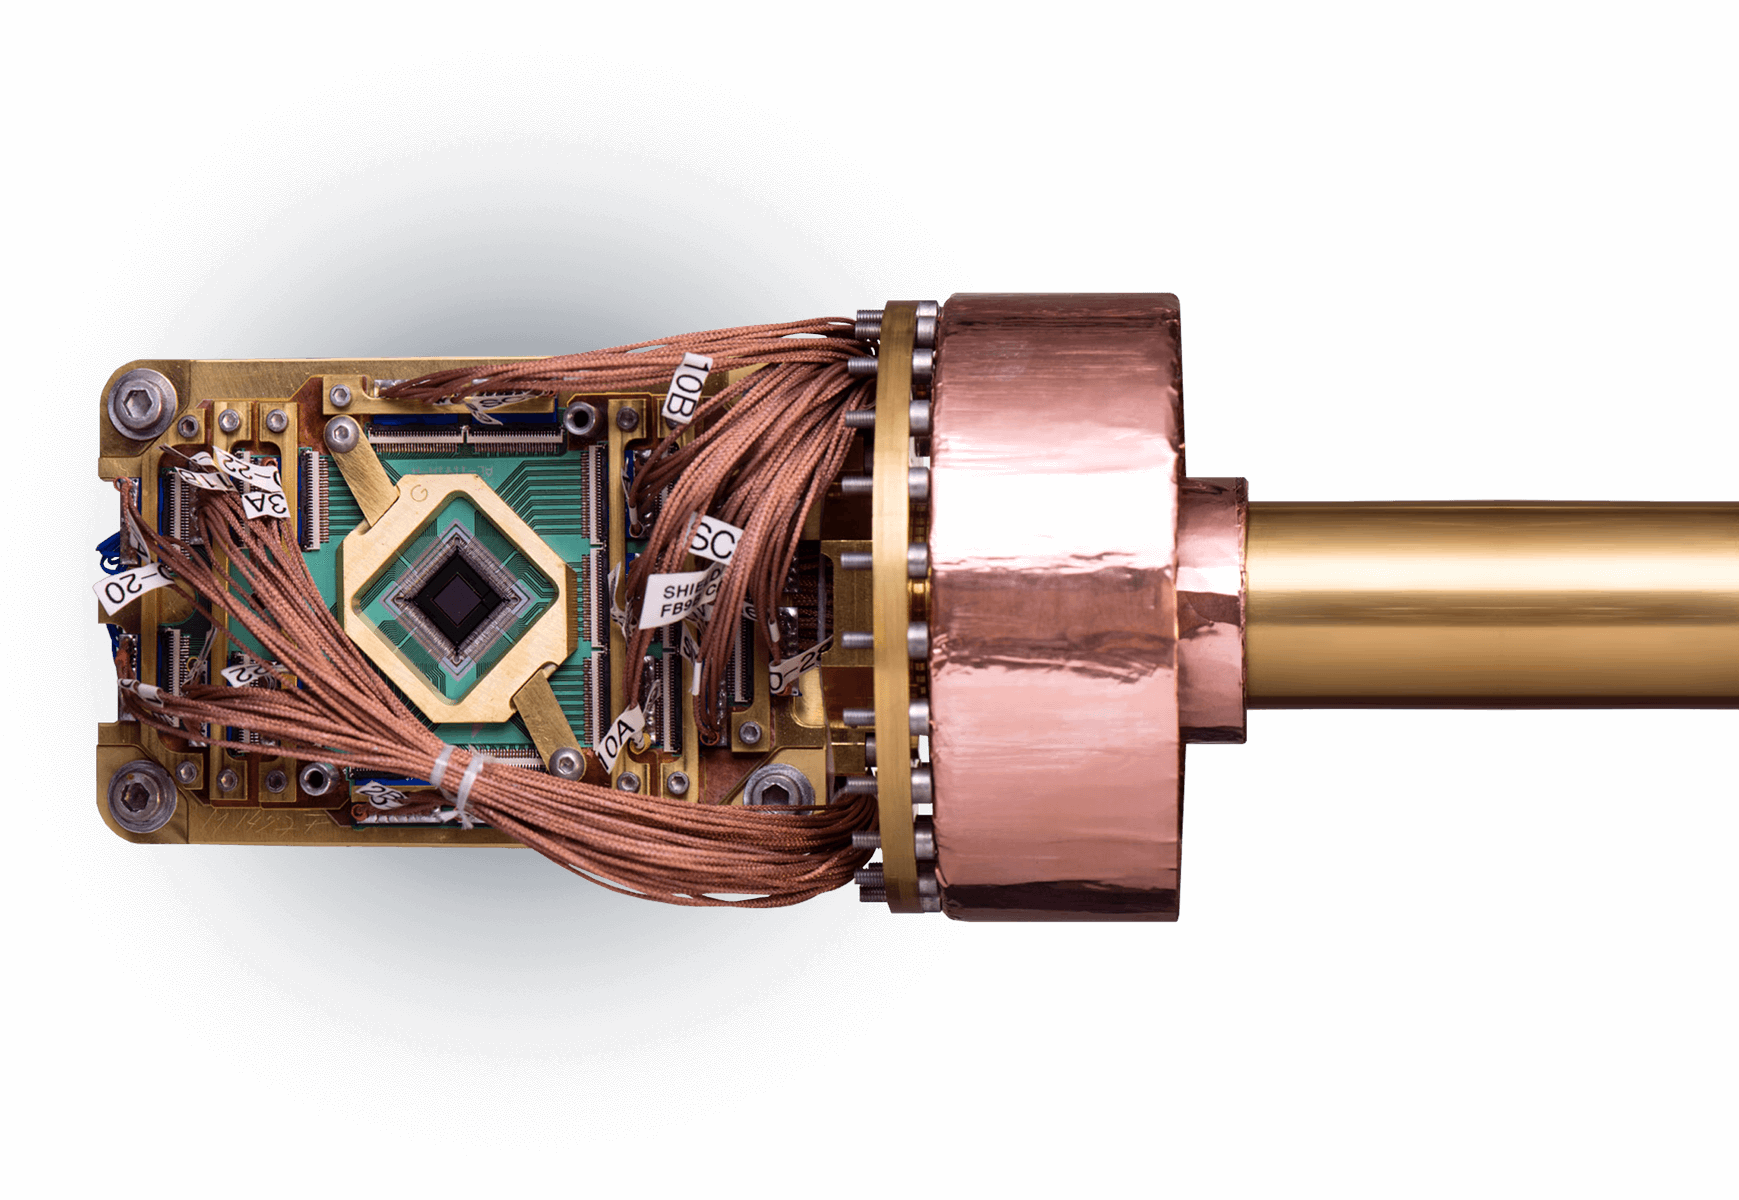
\includegraphics[width=0.9\textwidth]{../plots/dwave-chip.png}
            \end{figure}
            \vspace*{-3em}
            {\tiny \hspace*{2.2em} \texttt{https://quantumzeitgeist.com}}
        \end{column}
        \begin{column}{0.5\textwidth}
            \begin{itemize}
                \itemb D-Wave: superconducting qubits in a dilution refrigerator at $T \approx \SI{15}{\milli\kelvin}$
            \end{itemize}
            \begin{figure}[!htb]
                \centering
                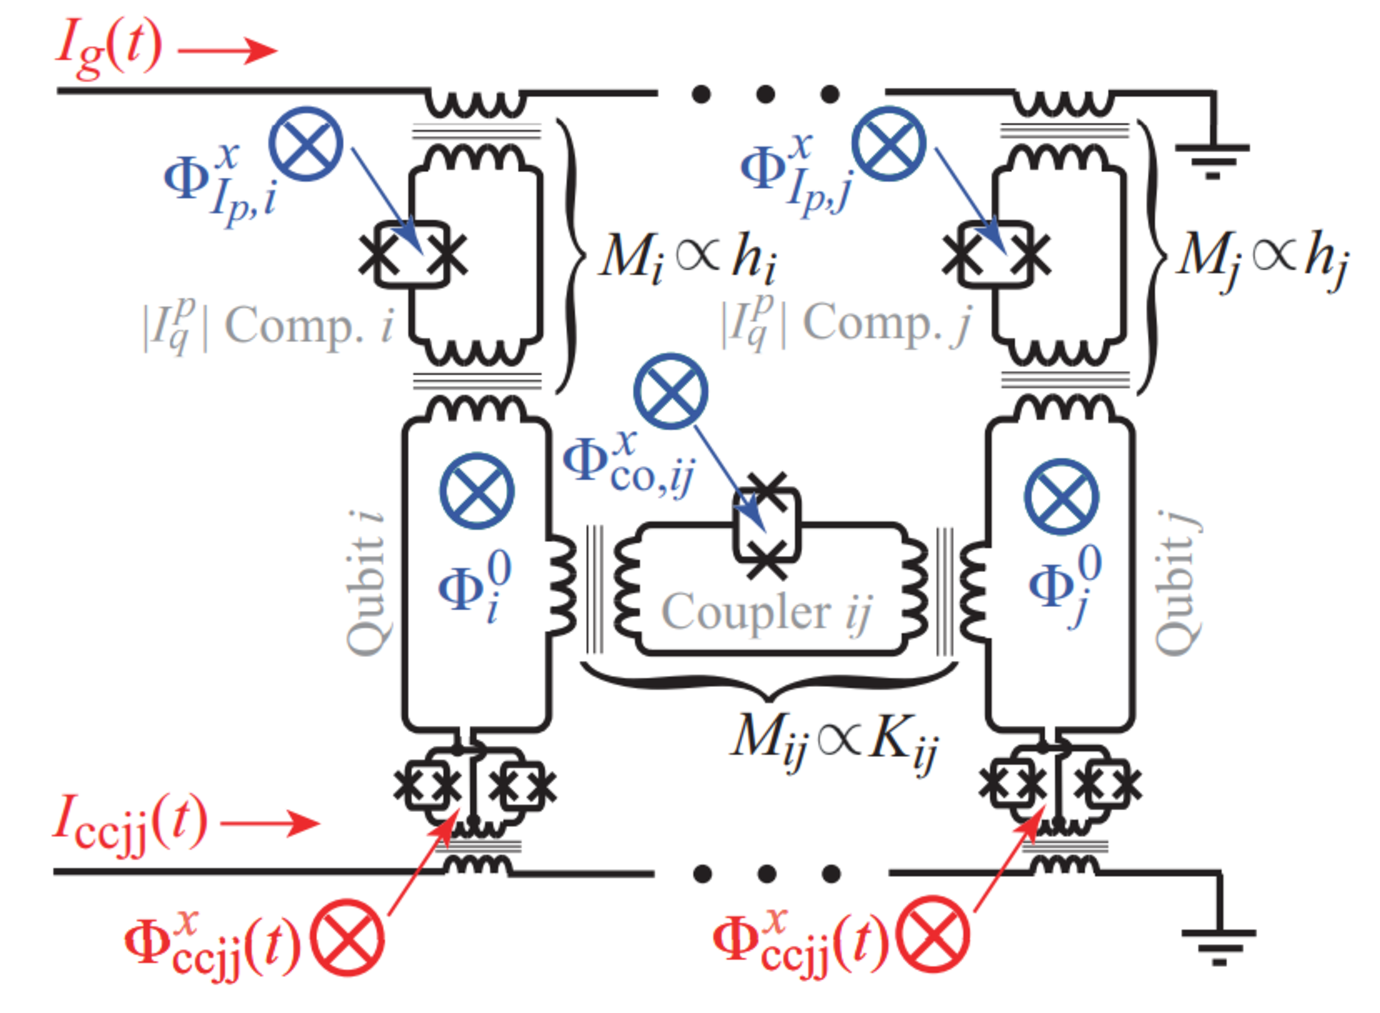
\includegraphics[width=0.9\textwidth]{../plots/sc_qubits_and_couplers.pdf}
            \end{figure}
            \vspace*{-0.5cm}
            {\tiny \hspace*{1.6em} Harris, R. et al. Phys. Rev. B (2010)}
        \end{column}
    \end{columns}
\end{frame}

\begin{frame}
    \frametitle{Sampling on quantum annealers}
    \begin{itemize}
        \setlength{\itemindent}{-1em}
        \itemb sampling workflow
        \vspace*{0.3em}
        \begin{enumerate}
            \setlength{\itemindent}{-1em}
            \item specify the problem
            \begin{itemize}
                \setlength{\itemindent}{-2em}
                \item [-] TFIM on the cubic lattice with $J_{ij} = J$ and $h_i = 0$
            \end{itemize}
            \item specify simulation parameters $T, A(s)/B(s)$
            \item map simulation parameters to programmable parameters $J, s$
            \item embed the lattice onto the hardware graph
            \item obtain samples from the quantum annealer
        \end{enumerate}
    \end{itemize}
\end{frame}

\begin{frame}
    \frametitle{Pause annealing schedule}    
    \begin{columns}[T]
        \begin{column}{0.45\textwidth}
            \begin{itemize}
                \itemb protocol for drawing samples from the Boltzmann distribution on quantum annealers
                \itemb quench too slow
                \begin{itemize}
                    \item [-] $E \tau / \hbar \sim 10^3$
                    \item [-] overestimation of magnetization
                \end{itemize}
            \end{itemize}
        \end{column}
        \begin{column}{0.55\textwidth}
            \begin{figure}[!htb]
                \centering
                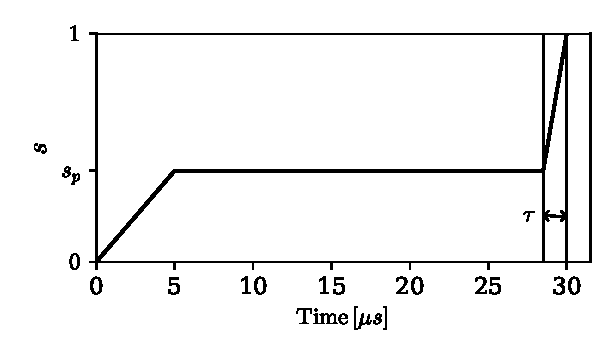
\includegraphics[width=\textwidth]{../plots/pause_schedule.pdf}        
            \end{figure}
        \end{column}
    \end{columns}
\end{frame}

\begin{frame}
    \frametitle{Magnetization overestimation}
    \begin{itemize}
        \setlength{\itemindent}{-1em}
        \itemb information about the slow quench imprinted in the samples
    \end{itemize} 
    \begin{figure}[!htb]
        \centering
        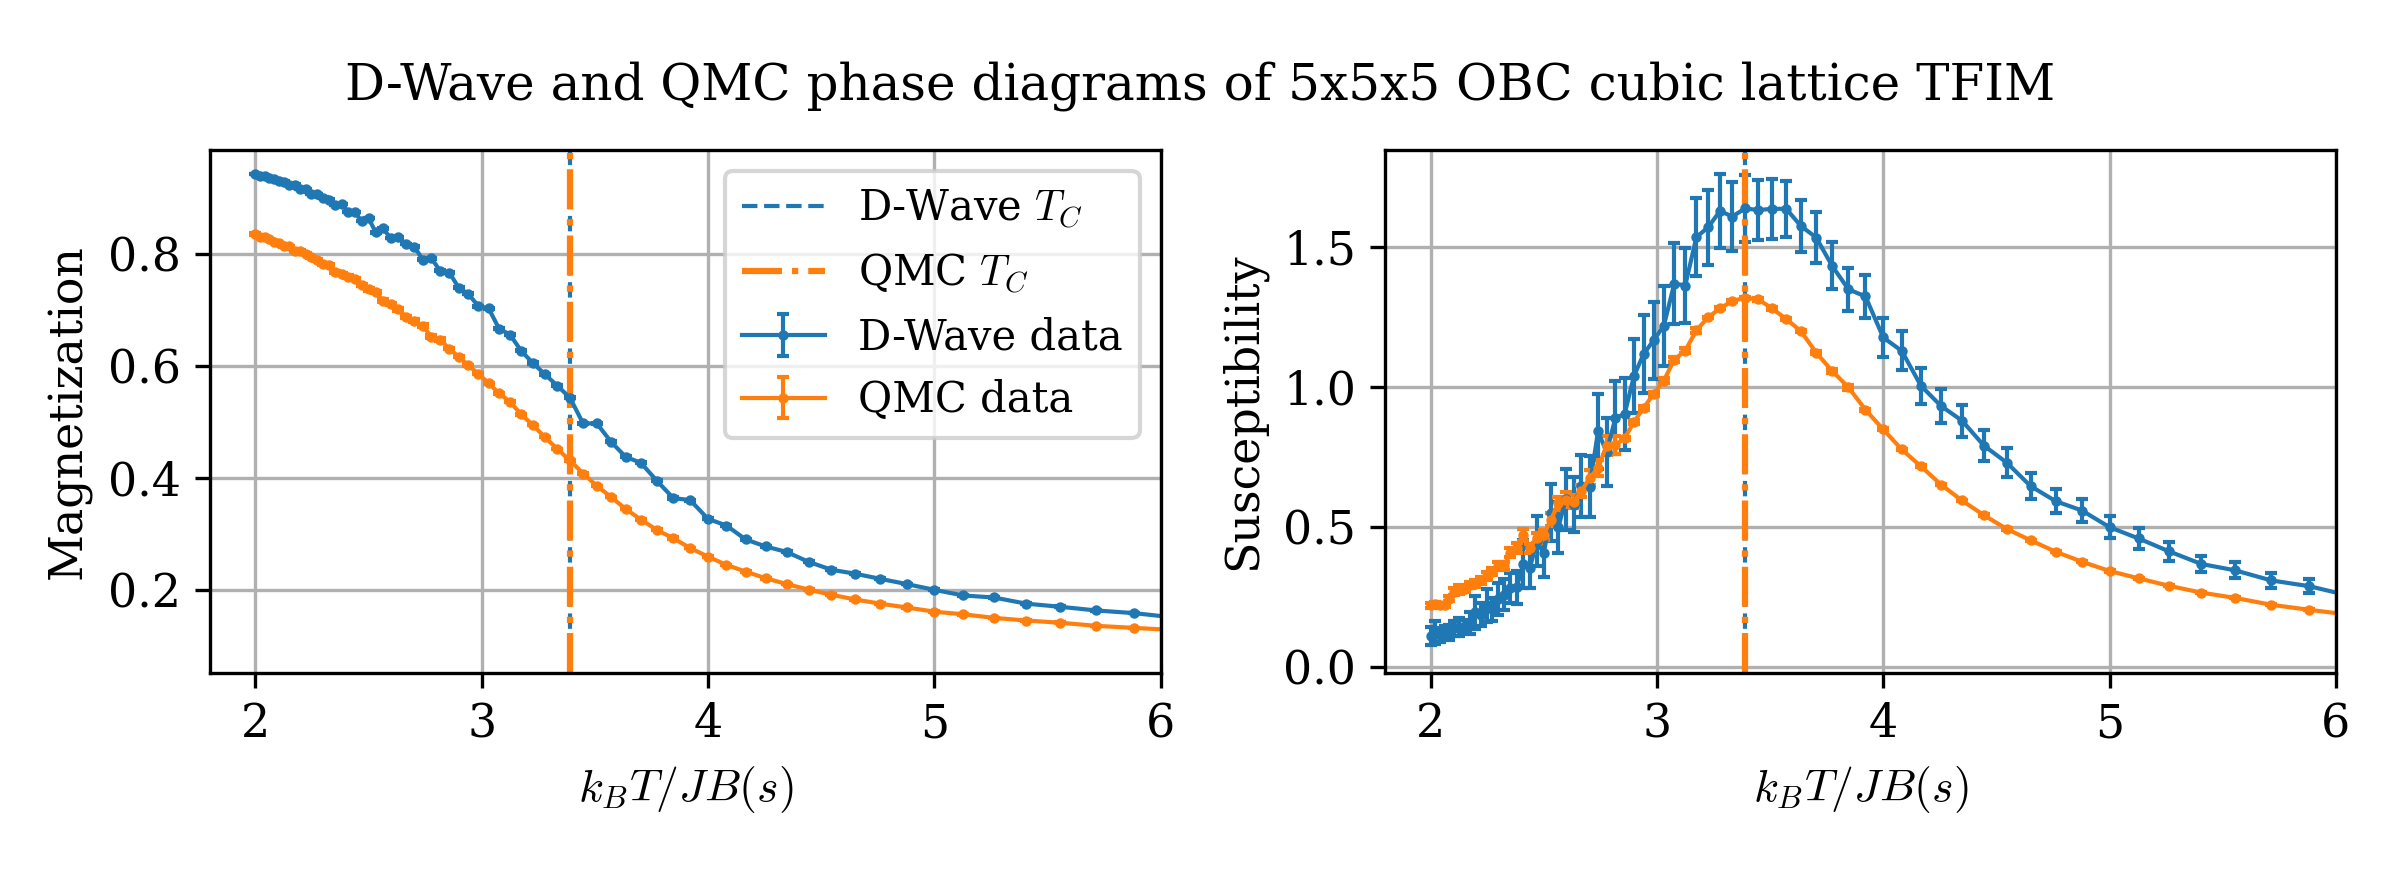
\includegraphics[width=0.9\textwidth]{../plots/dwave_vs_mcmc-5x5x5_gamma2.png}
    \end{figure}
\end{frame}

\begin{frame}
    \frametitle{Quantum Monte Carlo}   
    \begin{itemize}
        \setlength{\itemindent}{-1em}
        \itemb do annealers offer an advantage over classical methods?
        \itemb quantum Monte Carlo (QMC) methods: TFIM in $d$ dimensions
        \item [] = classical Ising model in $d+1$ dimensions
        \begin{itemize}
            \setlength{\itemindent}{-1em}
            \item [-] use Metropolis algorithm in $d+1$ dimensions
        \end{itemize}
        \itemb TFIM is \textit{stoquastic} (stochastic + quantum)
        \begin{itemize}
            \setlength{\itemindent}{-1em}
            \item [-] no negative transition probabilities between basis states
            \item [] $\ket*{000...}, \ket*{100...}, \ket*{010...}, \ldots$ $\implies$ TFIM simulable by a
            \item [] stochastic process
        \end{itemize}
        \itemb increase the computational power of QA by adding $\sigma^x \sigma^x$ terms
        \item [] to the Hamiltonian
    \end{itemize}
\end{frame}

\section{Conclusion}

\begin{frame}
    \frametitle{Conclusion}
    \begin{itemize}
        \setlength{\itemindent}{-1em}
        \itemb quantum annealer = universal analog quantum computer
        \begin{itemize}
            \setlength{\itemindent}{-1em}
            \item [-] specialized for optimization problems
            \item [-] exploited for quantum simulation
        \end{itemize}
        \itemb quantum simulation
        \begin{enumerate}
            \setlength{\itemindent}{-1em}
            \item equilibrium simulation
            \begin{itemize}
                \setlength{\itemindent}{-1em}
                \item [-] quantum annealers efficiently simulated with QMC methods
            \end{itemize}
            \item closed-system dynamics
            \begin{itemize}
                \setlength{\itemindent}{-1em}
                \item [-] no known efficient generally aplicable classical algorithm
                \item [-] shorter quench times make this possible on quantum annealers $\to$ quantum advantage
            \end{itemize}
        \end{enumerate}
    \end{itemize}
\end{frame}

\end{document}